% !TEX root = ../om_ts_03.tex

\begin{frame} % название фрагмента

\videotitle{Собери свой ETS!}

\end{frame}



\begin{frame}{Собери свой ETS: план}
  \begin{itemize}[<+->]
    \item Собираем ETS(MAdM) модель. 
    \item Прогнозы.
  \end{itemize}

\end{frame}


\begin{frame}
  \frametitle{Разная амплитуда колебаний}

  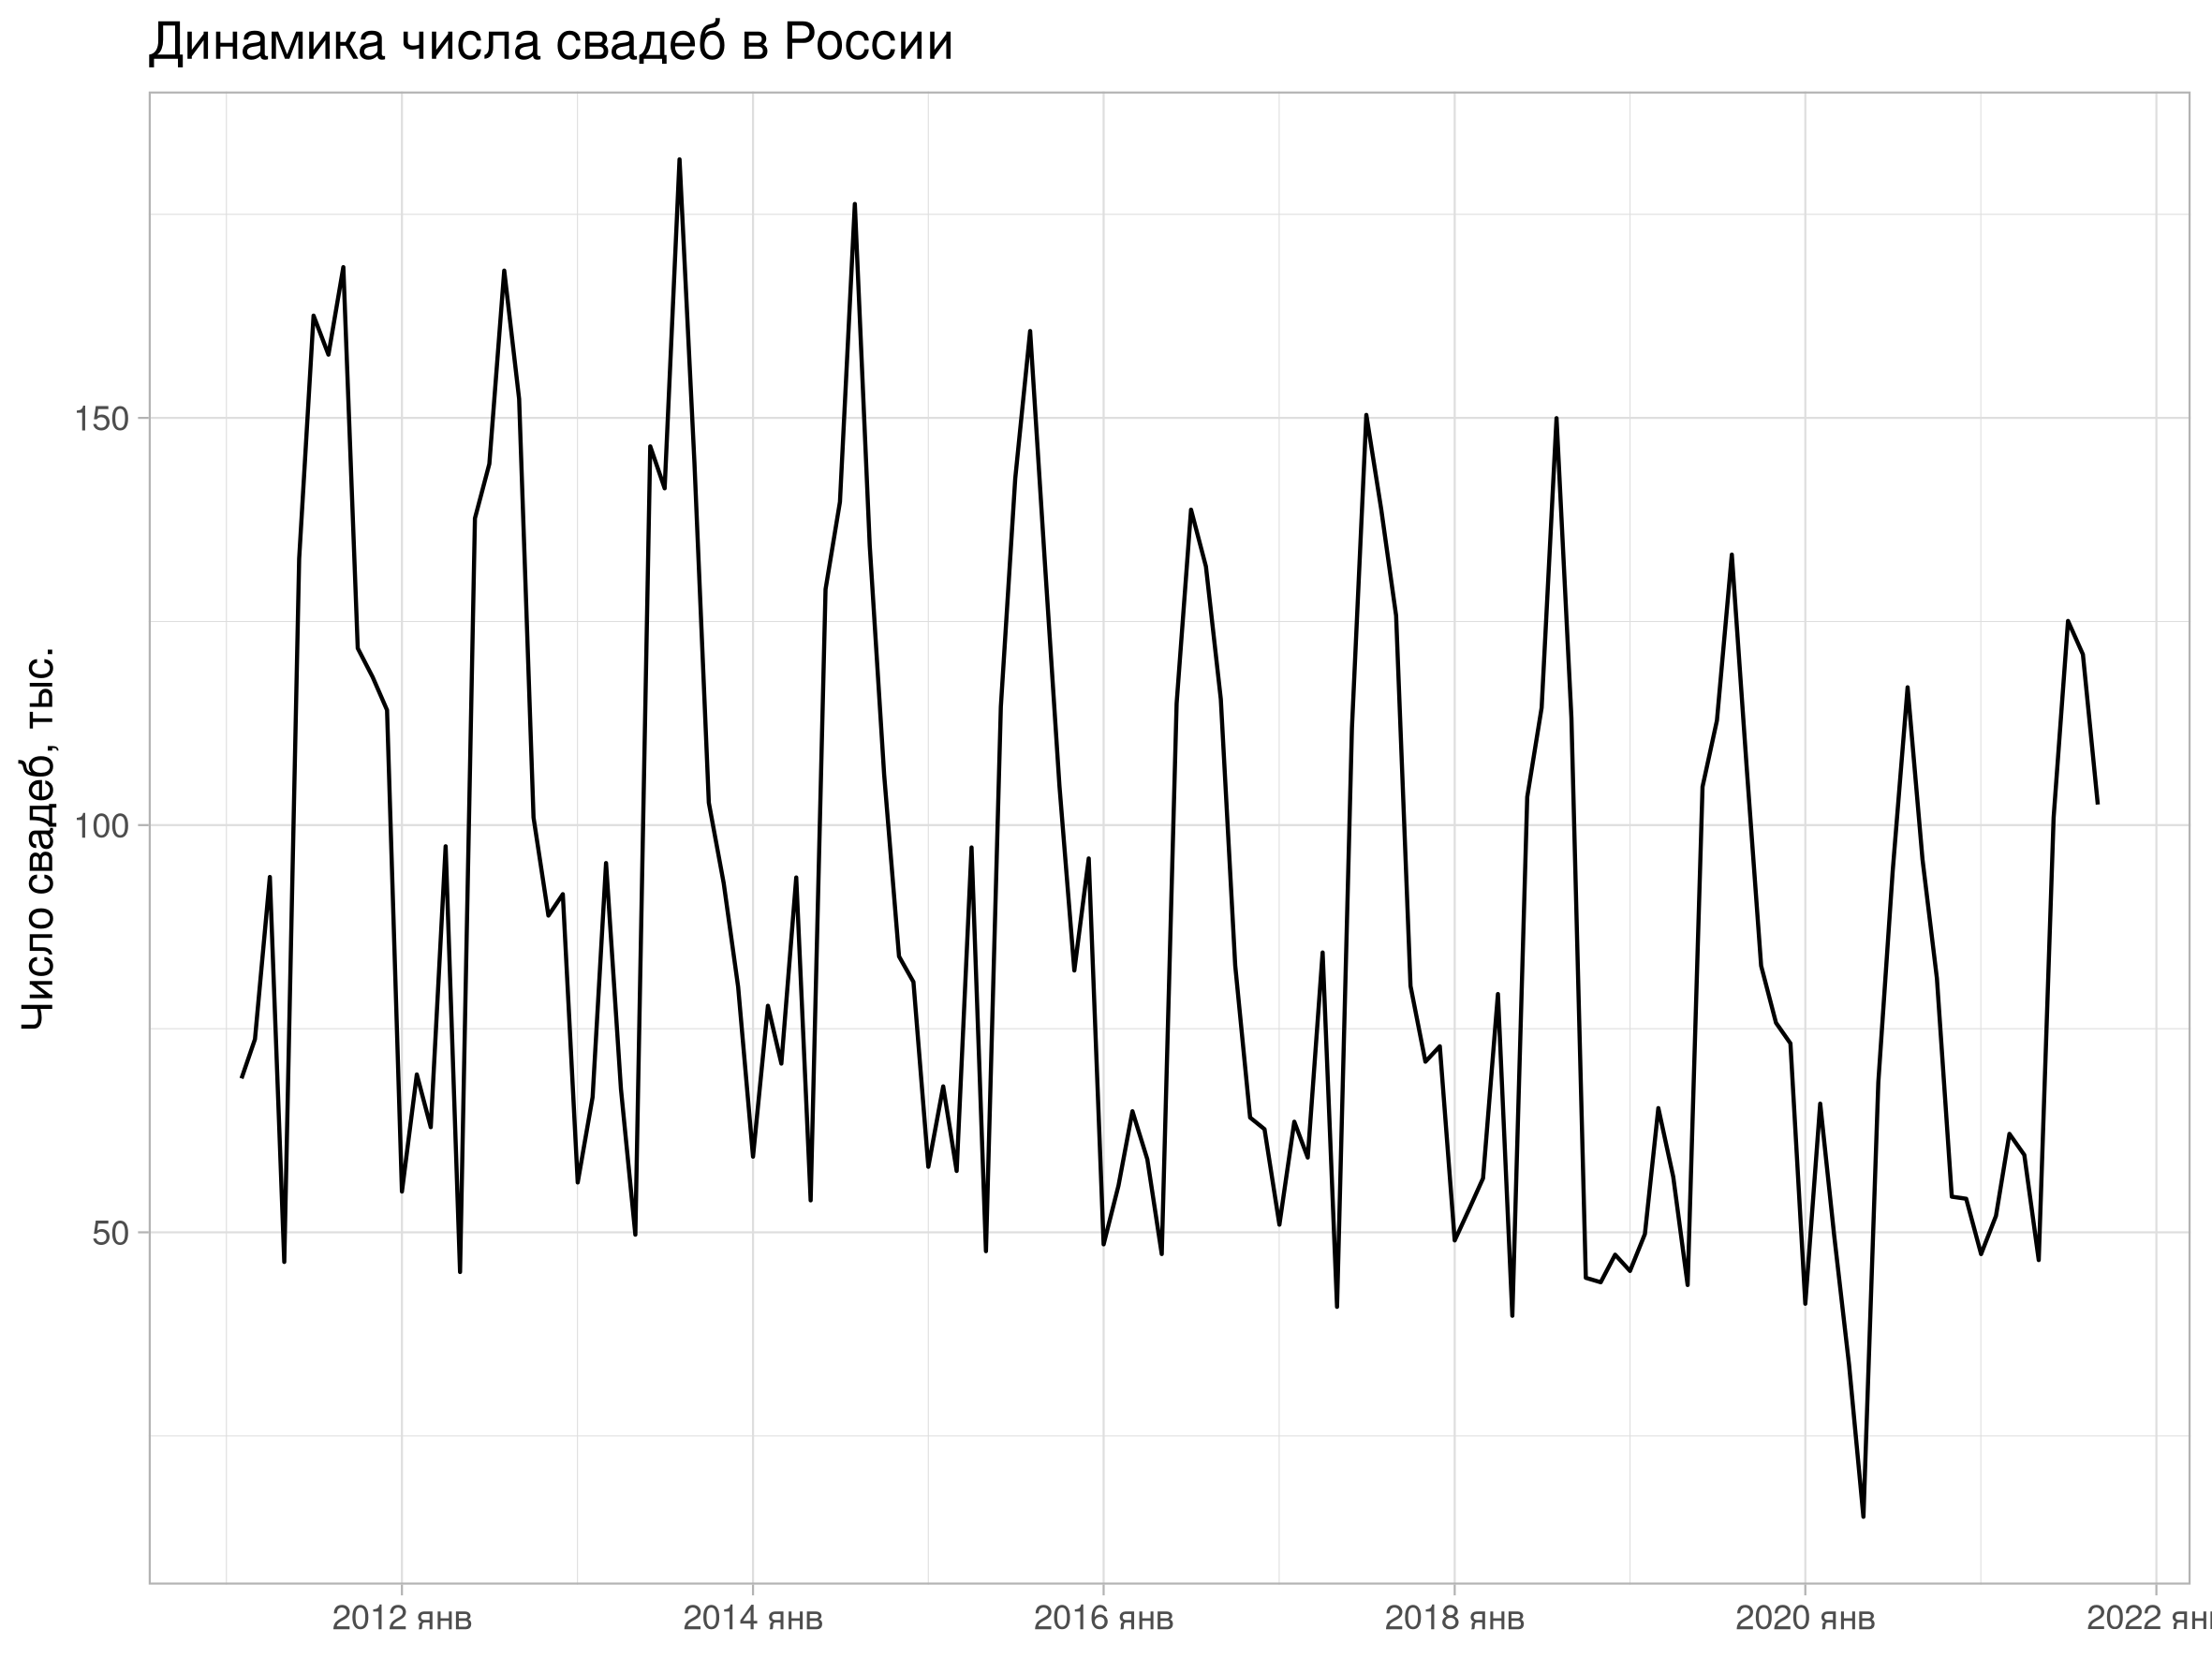
\includegraphics[width=\textwidth]{pictures/om_ts_03-060.png}


\end{frame}


\begin{frame}{Хочу разные компоненты}

Сезонность похожа на \alert{мультипликативную}.

\pause

Мультипликативный тренд означал бы \alert{экспоненциальный} рост.

\pause 

Хочу \alert{аддитивный} затухающий тренд.


\end{frame}


\begin{frame}
  \frametitle{ETS(MAdM): уравнения}

  ETS(MNM) для месячных данных:
  
  \[
    \begin{cases}
     y_t = \ell_{t-1} \cdot s_{t-12} \cdot (1 + u_t); \\
    \ell_t = \ell_{t-1}\cdot  (1 + \alpha u_t), \text{ стартовое } \ell_0; \\
    s_t = s_{t-12}\cdot (1 + \gamma u_t), \text{ стартовые } s_0, \ldots, s_{-11}; \\
    u_t \sim \dN(0;\sigma^2) \text{ и независимы.} \\
    \end{cases}
  \]

  \pause
  Как сюда добавить аддитивный тренд?
  \[
    b_t = \phi b_{t-1} + \beta u_t, \text{ стартовое } b_0.
  \]
\end{frame}


\begin{frame}
  \frametitle{ETS(MAdM): уравнения}

  ETS(MAdM) для месячных данных:
  
  \[
    \begin{cases}
     y_t = (\ell_{t-1} + \alert{\phi  b_{t-1}}) \cdot s_{t-12} \cdot (1 + u_t); \\
    \ell_t = (\ell_{t-1} +  \alert{ \phi  b_{t-1}}) \cdot  (1 + \alpha u_t), \text{ стартовое } \ell_0; \\
    \alert{b_t = } \phi  b_{t-1} + \beta (\ell_{t-1} + \phi  b_{t-1}) u_t, \text{ стартовое } b_0; \\
    s_t = s_{t-12}\cdot (1 + \gamma u_t), \text{ стартовые } s_0, \ldots, s_{-11}; \\
    u_t \sim \dN(0;\sigma^2) \text{ и независимы.} \\
    \end{cases}
  \]

  \pause
  Параметры — \alert{18 штук}.


\end{frame}


\begin{frame}
  \frametitle{ETS(MAdM): прогнозируем}

  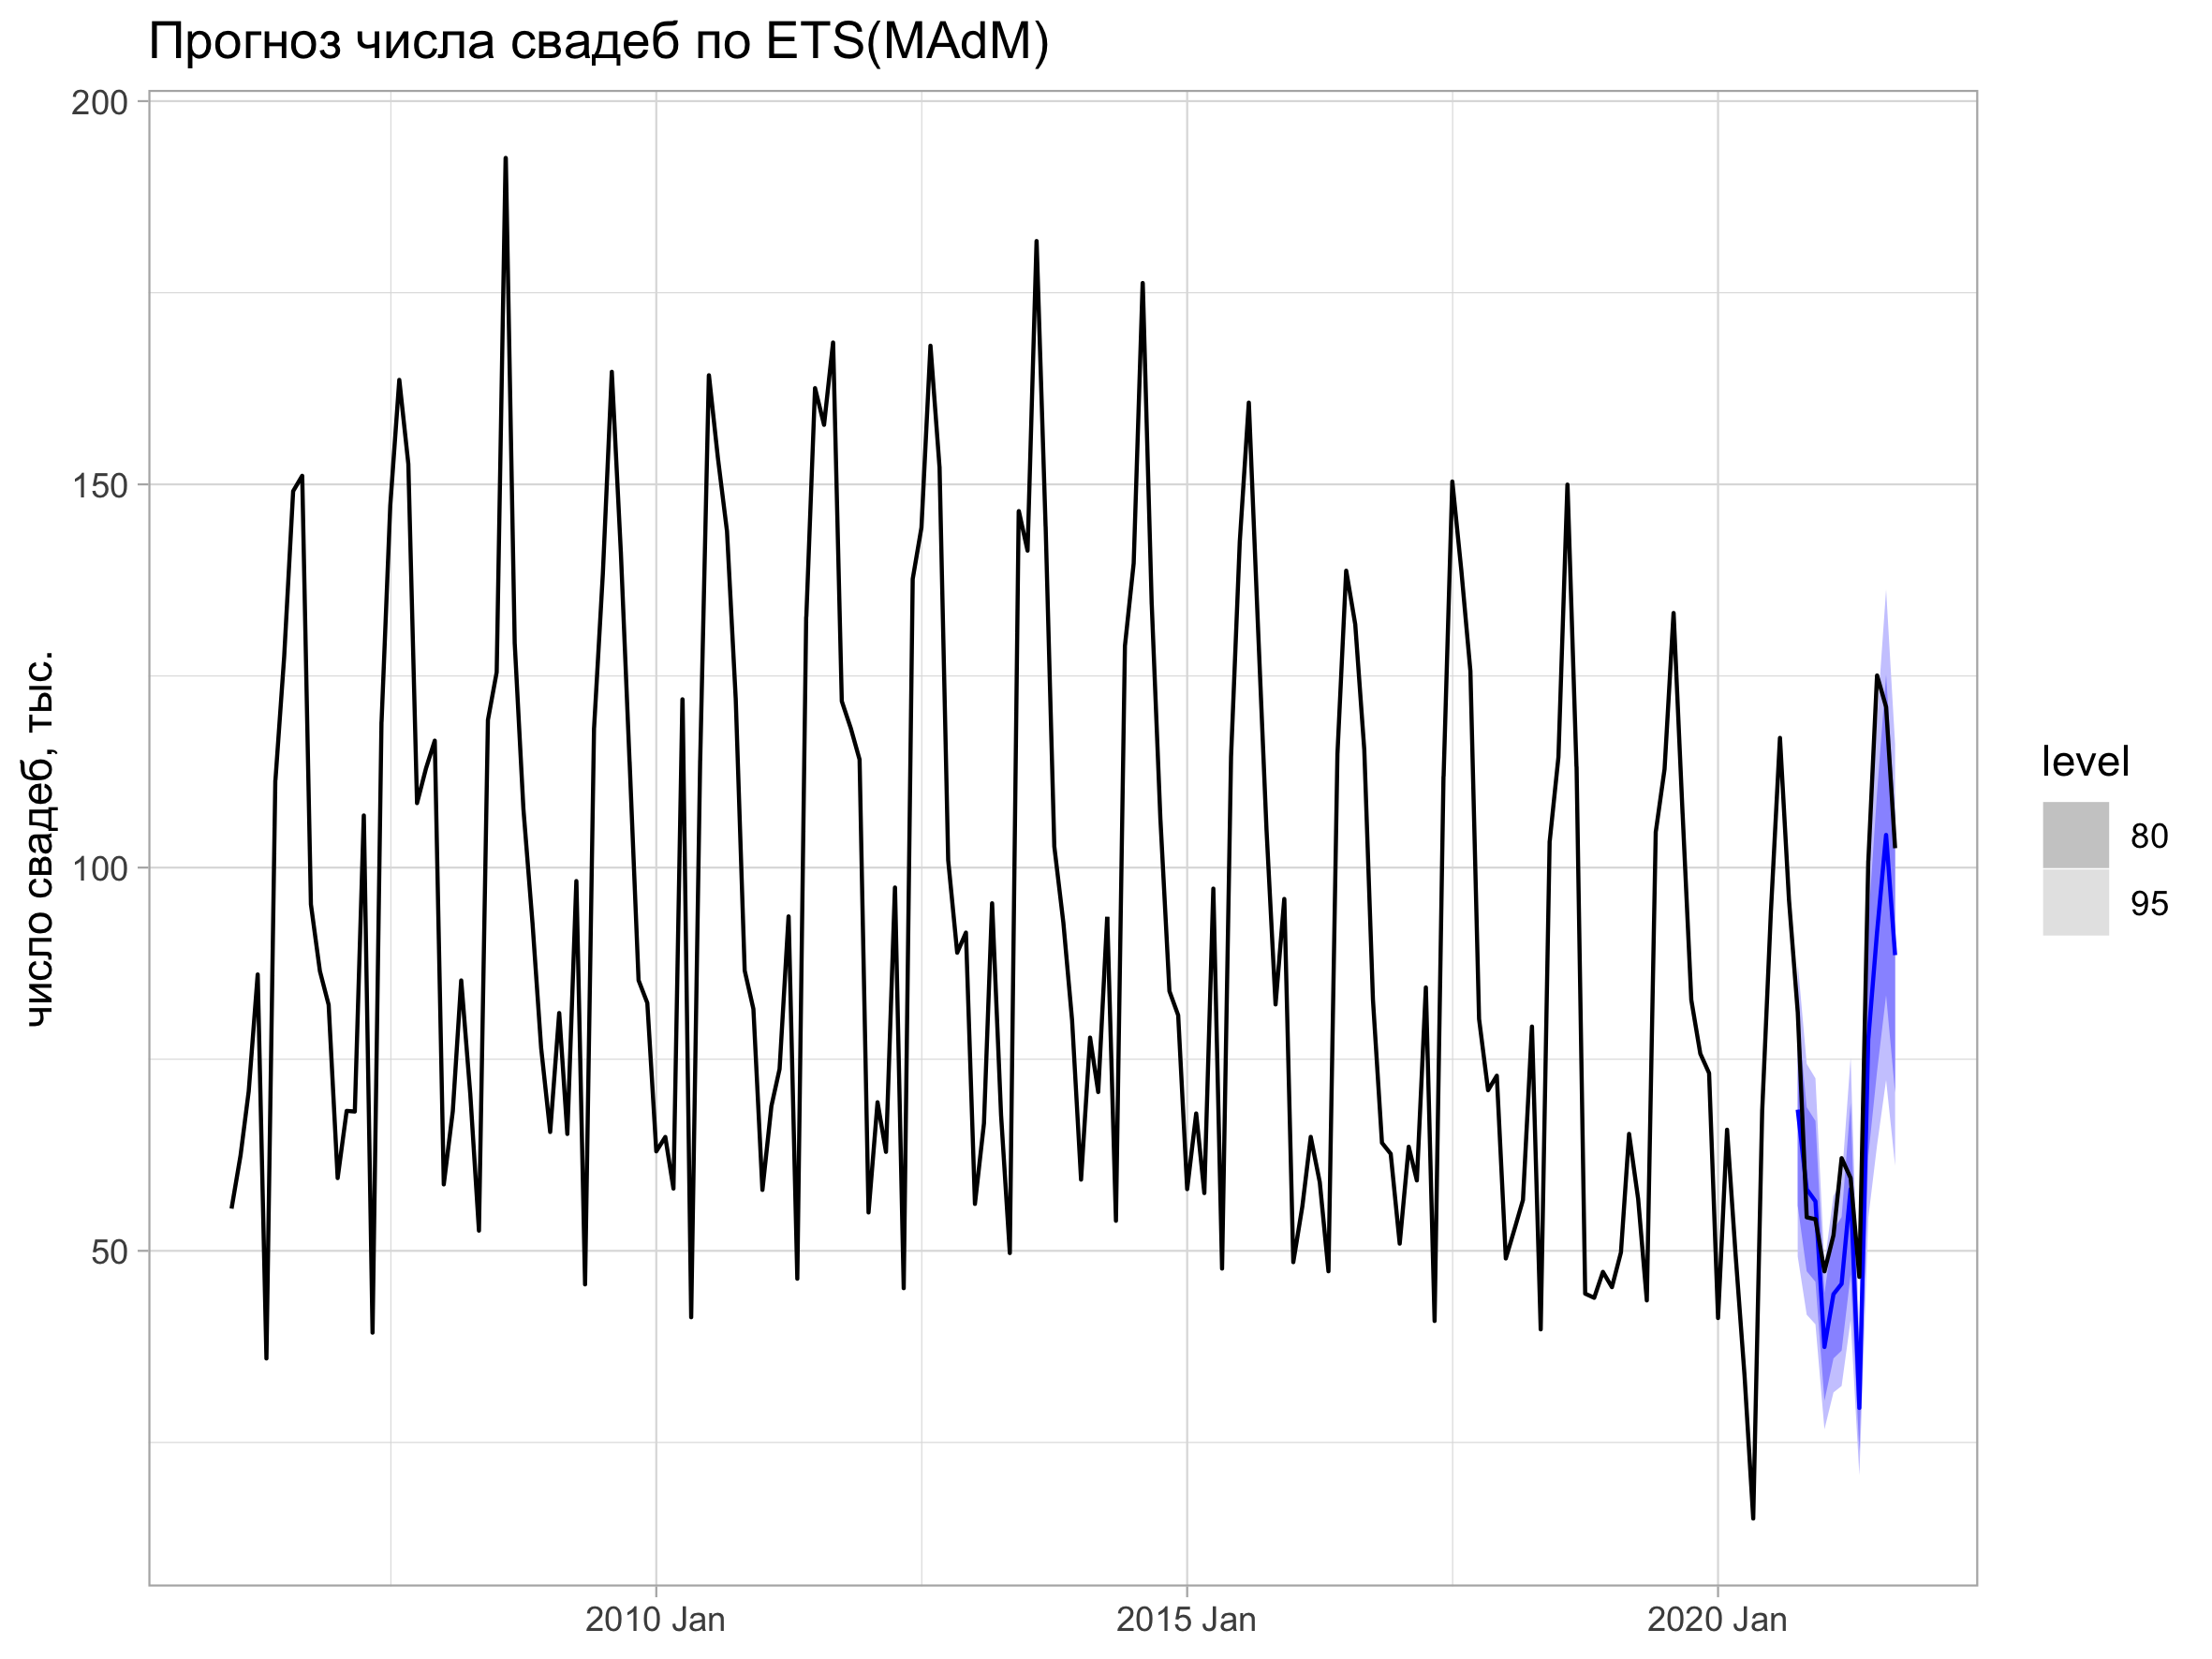
\includegraphics[width=\textwidth]{pictures/om_ts_03-068.png}


\end{frame}


\begin{frame}
  \frametitle{Прогноз на 1 шаг вперёд}

  \[
    \begin{cases}
     y_t = (\ell_{t-1} + \alert{\phi  b_{t-1}}) \cdot s_{t-12} \cdot (1 + u_t); \\
    \ell_t = (\ell_{t-1} +  \alert{ \phi  b_{t-1}}) \cdot  (1 + \alpha u_t), \text{ стартовое } \ell_0; \\
    \alert{b_t = } \phi  b_{t-1} + \beta (\ell_{t-1} + \phi  b_{t-1}) u_t, \text{ стартовое } b_0; \\
    s_t = s_{t-12}\cdot (1 + \gamma u_t), \text{ стартовые } s_0, \ldots, s_{-11}; \\
    u_t \sim \dN(0;\sigma^2) \text{ и независимы.} \\
    \end{cases}
  \]
  \pause
\[
y_{T+1} = (\ell_T + \phi b_T)\cdot s_{T-11} \cdot (1 + u_{T+1})  
\]
\pause
\[
  (y_{T+1} \mid \mathcal F_T) \sim \dN((\ell_T + \phi b_T) \cdot s_{T-11} ; (\ell_T + \phi b_T)^2 \cdot s_{T-11}^2\sigma^2)  
\]

\end{frame}




\begin{frame}
  \frametitle{Сколько всего ETS моделей?}

  
  \alert{Ошибка}: A, M.
  
  \alert{Тренд}: N, A, Ad, M, Md. 
  
  \alert{Сезонность}: N, A, M.

  \pause
  A — \alert{аддитивная} составляющая. 

  M — \alert{мультипликативная} составляющая. 

  N — нет составляющей. 

  d — \alert{дампирование} для тренда. 

  \pause

  Формально: \alert{30 вариантов}. 

\end{frame}


\begin{frame}{Исторические названия}

  ETS(ANN) — простое экспоненциальное сглаживание.

  ETS(AAA) — аддитивный метод Хольта-Винтерса.

  ETS(AAM) — мультипликативный метод Хольта-Винтерса.

  ETS(AAdM) — метод Хольта-Винтерса с затухающим трендом.
  
\end{frame}


\begin{frame}{Какой вариант выбрать?}

  \alert{Разная амплитуда} колебаний: признак мультипликативных моделей.

  \pause

  Работает автоматический выбор по критерию \alert{AIC}.

  \pause

  Часть мультпликативных моделей может быть \alert{численно неустойчива} 
  или \alert{не реализованы} в софте. 

\end{frame}


\begin{frame}{Собери свой ETS: итоги}

  \begin{itemize}[<+->]
    \item Можно смешивать разные компоненты. 
    \item \alert{Ошибка}: A, M.
    \item \alert{Тренд}: N, A, Ad, M, Md. 
    \item \alert{Сезонность}: N, A, M.
    \item Некоторые комбинации могут быть \alert{неустойчивы}. 

  \end{itemize}
\end{frame}



